\chapter[Pathways to food security in rural Burkina Faso: the importance of consumption of home-produced food versus purchased food]{Pathways to food security in rural Burkina Faso: the importance of consumption of home-produced food versus purchased food} %TOC then chapter title
\chaptermark{Pathways to food security in rural Burkina Faso} %Running head
\label{cha:chapter5}
\vspace*{\fill}
This chapter is based on:
\\
\\
% Full citation of the published (or submitted/in review) article

Fraval, S., Yameogo, V., Ayantunde, A., Hammond, J., de Boer, I. J. M., Oosting, S. J., van Wijk, M. T. (submitted). \textit{Food Security}


\newpage

\section*{Abstract}
The number of undernourished people and the risk of micro-nutrient deficiency remains high in sub-Saharan Africa (SSA). Decades of policy designed to reverse the trends of food insecurity have illustrated that the causal pathways of intervention to end-point outcomes, such as nutrition, are not necessarily straightforward. Utilising well-established proxies for food security, this study investigates the relative importance of different pathways to food security in two subtly contrasting communities in the Sahelian and Sudanian Savanna zones of Burkina Faso (n=400). In Yatenga province, approximately 31\% of households were classified as `severely food insecure' in the `lean' period. In contrast, over 83\% of households sampled in Seno province were classified as being `severely food insecure' in the lean period. There were statistically significant associations between food security indicators and off-farm income, farm income and production diversity. The source of income had significantly different associations with diet diversity in the two provinces. In Yatenga province, higher gross farm income in the absence of off-farm income was predicted to result in more diverse diets; in Seno province, however, gross farm income was only predicted to result in more diverse diets when households are also earning off-farm income. Our analysis shows that, households are most differentiated by income generating pathways to food security. This finding should not detract from the essential role played by home-produced foods in improving food security. Rather, market-orientated agriculture and production for home consumption, as shown by households in this study, can be combined as part of a more resilient livelihood strategy.

\newpage

\section{Introduction}

The decade long decline in global chronic undernourishment has been reversed in recent years. The prevalence of chronic undernourishment in sub-Saharan Africa (SSA) has returned to pre-2005 levels, equating to approximately 237 million people unable to meet their energy needs in 2017 (\citealp{FAO2018}). There is also a high risk of micro-nutrient deficiency in the broader population, termed `hidden hunger' (another important aspect of malnutrition). \citet{Joy2014} provide startling estimates of deficiency risks for calcium ({\textgreater}50\% of the African population), zinc (40\%), selenium (28\%) and iodine (19\%). The individual and societal implications for such nutritional gaps are borne disproportionately by the rural population, indicated by the consistently higher prevalence of stunting in rural SSA (\citealp{Green2016}).

Given the persistence of undernourishment and hidden hunger, nutrition specific and nutrition sensitive interventions have been implemented across SSA (\citealp{DePee2017}). Agricultural interventions have an intuitive link with the most nutritionally vulnerable of communities, particularly those with limited off-farm employment options. The causal pathways from intervention to end-point outcomes, such as nutrition, are less straightforward (\citealp{Carletto2017}). Increased incomes and energy availability, for example, are necessary for alleviating undernourishment, but not sufficient for addressing `hidden hunger' (\citealp{Schipanski2016}; \citealp{McDermott2015}; \citealp{Hoddinott2012}). A greater understanding of these pathways is needed, particularly given the UN's ambitious target of `zero hunger' by 2030 (as part of the Sustainable Development Goals) with the constraints of stagnating aid flows (\citealp{OECD2015}) and low levels of research and development spending in SSA (\citealp{Pardey2016}).

One challenge in assessing the pathways from agricultural intervention to nutrition outcomes relates to monitoring the food security status of the population. Evaluating food access and micro-nutrient deficiencies has traditionally been time-consuming and invasive. More recently, however, proxies have been introduced to enable wide-scale monitoring and evaluation. Food insecurity scales and diet diversity scores (to a greater extent) have been assessed against diet quality and adequacy ratios, and have emerged as reliable proxies (evident in \citealp{Rah2010}; \citealp{Saha2009}; \citealp{Coates2007}; \citealp{Savy2005}; \citealp{Steyn2006}; \citealp{Arimond2004}; \citealp{Torheim2004}). In the one case where `household diet diversity score' (HDDS) was not associated with diet quality or adequacy ratios, an association was instead identified with `household food insecurity of access scale/prevalence' (HFIAS/HFIAP; \citealp{McDonald2015}). As HFIAS/HFIAP and HDDS represent different aspects of food security, both metrics are adopted in the present study.

Utilising these proxies for food insecurity, a growing body of literature has taken shape around the question of what differentiates those that are food insecure from those that are more food secure in high risk communities around the world. \citet{Powell2015} provides a summary of six such studies that identify positive relationships between the diversity of crops cultivated and HDDS. More recently, several studies -- largely focused on SSA -- have explored these relationships in greater detail. The emerging areas of investigation have centered on the roles of subsistence and market-orientated agriculture and off-farm income in HFIAS, HDDS or nutrient adequacy ratios. Income, and thus purchased foods has been found to be highly associated with dietary diversity in the majority of these studies, whereas food from subsistence production, while also significant, had a limited relationship with dietary diversity (\citealp{Some2018}; \citealp{Bellon2016}; \citealp{Koppmair2017325}; \citealp{Luckett20152479}; \citealp{Sibhatu201510657}; \citealp{Snapp2015}; and \citealp{Dillon2014}). \citet{Jones2016} and \citet{MKaibi2015} in comparison, emphasised the positive relationship farm production has with food security indicators (diet diversity and micro/macro nutrient intake in \citealp{Jones2016}; nutrient adequacy ratios and HFIAS in \citealp{MKaibi2015}). In the most geographically diverse study to date, the role of farm production on food security was found to be of varying importance depending on market opportunities, and the relationship was found to be non-linear (\citealp{Sibhatu201510657}). In the existing literature, however, there is a limitation that the relationships between subsistence production, market-orientated agriculture and food security have been modelled indirectly and often at one or two points of time in the year.

This present study seeks to improve our understanding of the causal pathways to improved food security in vulnerable rural communities. We do so by characterising farm systems, household demographics and food security status in subtly contrasting communities in drought prone regions of Burkina Faso. Food security indicators were enumerated for two periods to account for the temporal variability throughout the year. Diet diversity was disaggregated by channel of access to better understand food sourcing behaviour. With this approach we address the questions of: a) what are the differentiating attributes of more food secure households, and more specifically b) what are the roles of subsistence and market-orientated agriculture in improving food availability, food access and the stability of food security.

\section{Methods}

\subsection{Household characteristics}

The two study areas are located in the Sahel and Sudanian Savanna zones of northern Burkina Faso. Elevation in these regions ranges from 250 to 350 masl., receiving between 300 and 600 mm of rainfall per year, in a unimodal pattern (based on publicly available GIS data). Soils in northern Burkina Faso are characterised as granite and migmatite derivatives, with poor soil fertility (\citealp{FAO2002}). We selected Seno and Yatenga provinces as our study areas as both provinces are vulnerable to food insecurity and have subtly contrasting production potential and ethno-cultural backgrounds.

The prevalence of chronic malnutrition in Burkina Faso remains of concern. According to a nutritional survey conducted in the country in 2016, the national prevalence of chronic malnutrition was estimated to be 7.6\% for all men, women and children (\citealp{MinistryofHealthBurkinaFaso2016}). This prevalence varied across the country, with 7.9\% of individuals in the region surrounding Seno identified as malnourished, and 8.2\% in the region surrounding Yatenga. Chronic and hidden hunger are experienced most severely in the lean period. The most food insecure period is during planting (typically June to August), where the lean period typically extends from May to mid-August -- with some variation across agro-ecological zones (\citealp{Some2018}). In general, diet diversity is lower in the Sahel and Sudanian Savanna zones compared the wider Burkina Faso (ibid.).

Households were sampled from eight villages in Seno and Yantenga provinces for this cross-sectional study (Figure \ref{map:05_1}). Both regions have good access to road infrastructure -- where major roads are paved and intra-village dirt roads are passable throughout the year. Each region has access to open air markets, where the average travel time for sampled households is approximately 10 kilometres. The largest livestock and produce market in Seno province is located in Bani; the largest livestock market in Yatenga province is located in Aorema, Ouahigouya. Households in Seno province are largely from the Fulani tribe, who have rich pastoralist and livestock keeping traditions. The Fulani pastoralists in the study area have largely been sedentarised for the past three generations. Some households in the region settled more recently due to loss of their animals during the droughts of the 1970s and 1980s (\citealp{Bovin1990}). These recently sedentarised households tended to establish communities on the periphery of villages. Households in Yatenga province are largely of the Mossi tribe, which is the largest ethnic group in the country.

\begin{figure}
  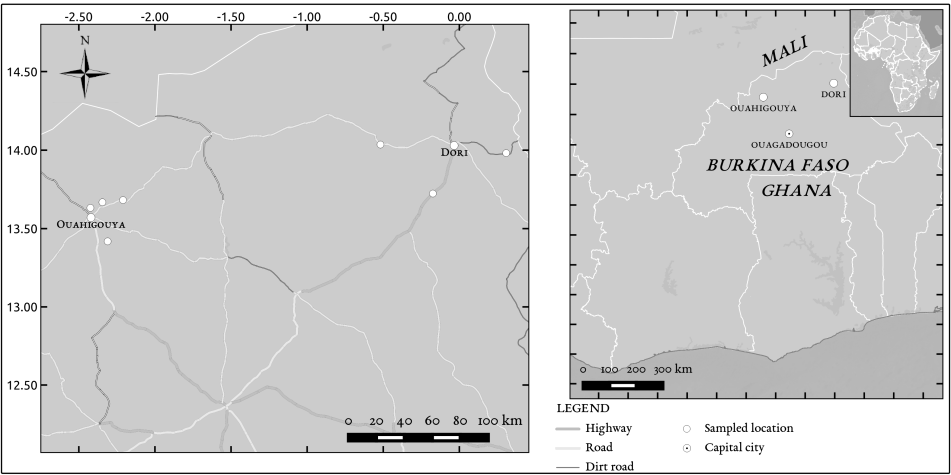
\includegraphics[width=0.9\textwidth]{figs_05/image1.png}
  \captionsetup{singlelinecheck = false, justification=justified}
  \caption{Study areas and sampled villages}
  \label{map:05_1}
  %\small
  %\raggedright
  \vspace*{-3mm}
  \caption*{(Author's composition based on GADM database and Open Steet Maps)}
\end{figure}



Households in both provinces rely largely on rain-fed agriculture. According to the \citet{GlobalYieldGapAtlas2016}, both provinces fall below their potential in terms of crop production. The rain-water limited yield potential in Dori was 2.7 tonnes per hectare for \textit{sorghum} (\textit{bicolor}) and 1.3 tonnes per hectare for millet (predominantly \textit{Pennisetum glaucum L.} possibly also \textit{Eleusine coracana L}), with actual yields estimated to be below one tonne per hectare; water limited yield potential in Yatenga was estimated to be 5.5 tonnes per hectare for sorghum and 2.7 tonnes per hectare for millet, with actual yields also estimated to be below one tonne per hectare.

\subsection{Data}

Fifty households were randomly sampled from four villages in each region, totalling 400 households. Villages were selected based on the following criteria: i) representativeness (e.g. ethnicity, wealth, scale of production), ii) population (at least 500 households), iii) suitability for on-farm trials, and iv) security risk (northern departments/communes in Yatenga were excluded on this basis). Focus group discussions were conducted in the eight villages, each including 20 to 25 participants. Households were then randomly sampled based on full lists of households -- provided by the village leaders. Due to limitations on pre-existing data, sample size was set at 50 households per village -- based on an approximate target of 5 - 10\% of the population (\citealp{Lapan2011}; village household population is presented in Table \ref{tab:05_1}). All selected households agreed to participate. The interview questions were developed based on objectives for the project and the research questions of this study. The questionnaire was pre-tested in each village to ensure the questions were appropriately framed.

Data collection took place in May 2016, administered in French and in local languages when preferred (Fulfulde in Seno province and Moore in Yatenga province). Interviews were conducted by trained enumerators at the respondent's homestead. The household head responded to the majority of questions and other household members were engaged on questions related to food security (e.g. the person who prepares the meals). Respondents were asked detailed questions on household demographics, plot utilisation, livestock holdings, crop yields, farm product utilisation, income, diet, food security, poverty level and labour allocation. Households were asked to recall circumstances from both the most food secure period and the least food secure period of the year (the periods of challenged food security are defined by respondent perceptions of scarcity and presented in the results).

\begin{table}[b]
  \captionsetup{singlelinecheck = false, justification=justified} %left justify caption
  \caption{Number of households by department and village}
  \label{tab:05_1}
  \small
\begin{tabularx}{\textwidth}{@{}lllYY@{}}
  %{
%p{\dimexpr 0.11\linewidth-2\tabcolsep}
%p{\dimexpr 0.25\linewidth-2\tabcolsep}
%p{\dimexpr 0.12\linewidth-2\tabcolsep}
%p{\dimexpr 0.28\linewidth-2\tabcolsep}
%p{\dimexpr 0.23\linewidth-2\tabcolsep}}
\toprule
Province & Department / commune & Village & Households in department${\dag}$ & Households in village${\dag}$ \\
\midrule
Seno & Bani & Bani & 12,102 & 1,030 \\
 & Dori & M'Bamga & 21,366 & 655 \\
 & Gorgadji & Gorgadji & 5,554 & 823 \\
 & Seytenga & Seytenga & 6,102 & 851 \\
Yatenga & Ouahigouya & Aorema & 22,091 & 578 \\
 & & Bogoya & & 879 \\
 & Namissiguima & Tougou & 6,754 & 687 \\
 & Oula & Ziga & 5,536 & 610 \\
 \bottomrule
\end{tabularx}
\footnotesize
\raggedright
%\caption*{
${^\dag}$Census 2006%}
\end{table}



The core indicators assessed in this study were based on from standardised methodologies. `household food insecurity access prevalence' (HFIAP) and `household food insecurity access scale' (HFIAS) were calculated based on the nine food access questions from the `Food And Nutrition Technical Assistance' project (FANTA) guidelines (\citealp{Coates2007}), based on generalised recall of conditions in the `flush' and `lean' periods (full results tabulated in Appendix Table \ref{tab:B1}). `Household diet diversity scores' (HDDS) were calculated using a 12 food category scale as detailed in the FANTA guidelines (\citealp{Swindale2006}), based on recall of both periods. The recall period used in this study are an adaptation of existing guidelines, which suggest using 24-hour recall. This adaptation is designed to provide a more consistent metric -- independent of the timing or duration of survey implementation. The `flush' and `lean' periods of the study were relative to the individual household, where a household could be `food secure' but still report on the most lean period in the year. The indicator was also adjusted to enumerate the channel of HDDS categories (own-farm or purchased).

We calculated several variables on the household for the purpose of our analysis. These variables included the number of inhabitants and nutritional adequacy ratios. Adult equivalents were calculated based on energy requirements relative to adult female and males (averaged) between 25 and 50 (2500 kcal based on energy requirements from \citealp{FoodandAgricuturalOrganization2001}; \citealp{ClaroRafael2010}). Energy adequacy ratios were calculated for home consumed crop and livestock products and protein adequacy ratios were calculated for livestock products only -- based on food composition tables specific to west Africa (\citealp{FAO2012}) -- and a coarse measure of daily energy (2500 kcal adult equivalent$^{-1}$ day$^{-1}$) and protein requirements (56 g adult equivalent$^{-1}$ day$^{-1}$).

Variables calculated to characterise the farm and livelihoods of rural households included: farm production diversity, farm practice adoption, livestock holdings, crop yields, market participation, income, cost of production, gendered control of income and wealth. Farm production diversity has been represented several different ways in the literature (e.g. species count in \citealp{Bellon2016} and \citealp{MKaibi2015}, diet diversity aligned categories in \citet{Koppmair2017325} and \citet{Jones2016} and the debate between the approaches found in the dialogue between \citealp{Berti2015} and \citealp{Sibhatu201510657}). In the present study, we included a measure of crop and livestock diversity (count of species) and production diversity scores (count of products in the HDDS categories). A limitation of the production diversity scores is that they do not capture transformed crop and livestock products (e.g. into fats/oils).

Crop and livestock practice adoption was enumerated for each household, including adoption of irrigation, fertilisation, `improved' seeds, exotic breeds and value addition (adoption rates presented in Appendix Tables \ref{tab:B2} and \ref{tab:B3}). Livestock holdings were represented as Tropical Livestock Units (TLUs; conversion factors from \citealp{Njuki2011a}). Yields for sorghum, millet and maize were calculated based on farmer reported harvest volumes and area planted. Crop market participation was represented as the proportion sold of the total calorific value of crops produced; livestock market participation was represented as the proportion sold of total protein produced from livestock products. The profitability of agricultural enterprises was calculated using respondent estimated cost of production (COP) values where possible (live animals and livestock products), otherwise gross income was reported (crops). Gendered control of income was represented as the percentage of total income that females have autonomous control over. The `progress out of poverty index' (PPI) was calculated from 10 country specific questions on ownership of assets, education and household composition (\citealp{Schreiner2011}).

The cost of production for crops was impacted by item non-response. Due to the high instance of missing data (63\% of crops produced missing) it was not possible to impute these data. The result of this is that crop income is reported in this study as gross income, while livestock income is reported as net income. The proportion of crops sold was only enumerated for species that were marketed, as such missing values were instances where the proportion sold was zero.

\subsection{Statistical analysis}

Our analysis was undertaken in a step-wise manner to describe the potential pathways from intervention to improved food security. We assumed that food insecurity of access and diet diversity are determined by on-farm production and by off-farm sourcing through purchase (i.e. excluding hunting and foraging as there is little scope to intervene in these domains). We therefore first assessed the determinants of food security of access status (HFIAP), followed by the determinants of the on-farm and purchased channels of diet diversity. We also assessed to what extent intensification options are practiced by farmers.

Relationships between core indicators and independent variables were modelled using Bayesian regressions, with random effects from village groupings on the intercept. Regressions were weighted based on village populations to correct for over or under representation in some villages -- i.e. the sum of weightings equated to the sample size for each province. Multinomial regressions were used to model HFIAP, with the least desirable food security outcome as the reference category. Household diet diversity scores were modelled using negative binomial regressions to model the overdispersion in the HDDS variable (i.e. variation not equal to the mean; \citealp{McElreath2016}). Differences between groups were also modelled using a specification equivalent to a t-test, but without assumptions of normality (\citealp{Kruschke2013}).

Models were built in an additive fashion, assessing all potential variables that could influence food security or diet diversity. Priors for the beta coefficients were informed by field knowledge of the interaction of farm and household variables with food security. These prior distributions were informative to the extent that the explanatory variables were expected to be positively associated with food security; these priors were weakly informative in the sense that the ranges of plausible beta coefficients were not restricted. Student's t-distributions were used to this effect, with the mass of the prior distribution being centred to reflect a positive association (centred at 0.5), and the tails thicker than a normal distribution (df = 1) to allow for a greater range of plausible values. If for example, we were to use an exponential prior distribution on beta coefficients for HDDS we would constrain the posteriors to a floor of zero and an unconstrained upper ceiling. This could be reasonable if we are confident that the explanatory variables have a positive relationship with the dependent variable -- however, we have not constrained the models in such a way.

Models were chosen by minimising the Watanabe-Akaike Information Criterion (WAIC). Specifically, this means that if a variable is theorised to influence food security but is not significant in our models, then we only retain it if the WAIC is minimised. Further, convergence was assessed using trace plots, and the model's output Rhat, with chains and iterations adjusted as necessary.

Regressions were implemented in R using the `BRMS' package (v 1.0.1; \citealp{BuerknerP2016}). The `BRMS' package compiles Stan code (http://mc-stan.org/), which uses a hybrid Monte-Carlo Markov Chain (MCMC) method to approximate the posterior distribution of the desired conditional probabilities. Thus the logistic regression models estimate the log odds of an observation being in the higher performing category as opposed to the poorest performing category (severely food insecure) given a unit change in an independent variable, with random effects at the village level; the negative binomial models estimate the log of the expected counts holding all else constant.

\section{Results}

\subsection{Household characteristics and welfare in the two provinces}

There were significant differences in the livelihoods of households between the two provinces. Table \ref{tab:05_2} compares provinces based on variables related to livelihoods that have the potential to influence human nutrition. These variables are presented in the table as follows: resources (adult equivalents, land and livestock ownership), income (including gendered control), wealth (PPI), crop production (diversity, yields, market participation and energy adequacy), and livestock production (diversity, market participation and protein adequacy). There were notable differences between provinces in household demographics, land and land use, market participation, energy/protein adequacy, and income (significant differences indicated in column 4 of Table \ref{tab:05_2}). This section describes the variability and differences in livelihoods.

Household demographics differed across the two provinces. Households in Yatenga province tended to have more inhabitants and therefore, greater potential labour availability and marginally higher nutritional requirements. The household head in Yatenga province was generally older (${\upmu}$ = 57, sd = 12) than in Seno province (${\upmu}$= 50, sd = 13; results not shown), and for the vast majority ({\textgreater} 93\%) of households in both provinces, the household head was male (results not shown).

Households in Yatenga province had larger parcels of land (median of 5 ha) than in Seno province (3.5 ha; Table \ref{tab:05_2}), and the majority of households in both provinces utilised their land for mixed crop-livestock systems. Livestock holdings were similar across provinces, with medians of approximately five Tropical Livestock Units (TLUs); five households in Seno province, however, kept between 25 and 85 TLUs (results not shown). Land was cultivated in the `flush' period with sorghum and millet by almost all farmers; cowpeas (\textit{Vigna unguiculata L.}) were cultivated by the majority of farmers (99\% in Yatenga and 68\% in Seno); sesame (\textit{Sesamum indicum L.}) and maize \textit{(Zea mays L.}) was cultivated by approximately a quarter of farmers; groundnut (\textit{Arachis hypogaea L.}) was cultivated by the majority (96\%) of households in Yatenga province and some households in Seno province (9\%); rice (\textit{Oryza spp.}) production was exclusively in Yatenga province, largely in the Oula department. Vegetable cultivation was also more prevalent in Yatenga, with 20\% of households cultivating up to 1.5 hectares (results not shown). As such, there was greater crop diversity in Yatenga province when compared to Seno province (Table \ref{tab:05_2}).

Yields per hectare of staple crops were lower than the rain-water limited yield potential. Maize was the highest yielding staple crop, followed by the more commonly cultivated staples of sorghum and then millet. Crop yields for these three staple crops were marginally higher in Seno when compared to Yatenga (difference in millet yield was not statistically significant; Table \ref{tab:05_2}). Households differed in their levels of practice adoption. Improved seeds, fertiliser and irrigation were more readily adopted in Yatenga province; and, value addition was common in both provinces. As a proxy for the diversity of cash crop yield differences, Figure \ref{fig:05_1} presents crop income by adopted practices and province. Crop income was significantly higher for households in Yatenga province that adopted irrigation, fertilisers and/or improved seeds (Wilcoxon rank sum test; r = 0.51, 0.20 \& 0.28 respectively; p {\textless} 0.01). In terms of livestock, there was a low level of adoption of improved livestock breeds in both Seno and Yatenga provinces.

\begin{figure}[H]
  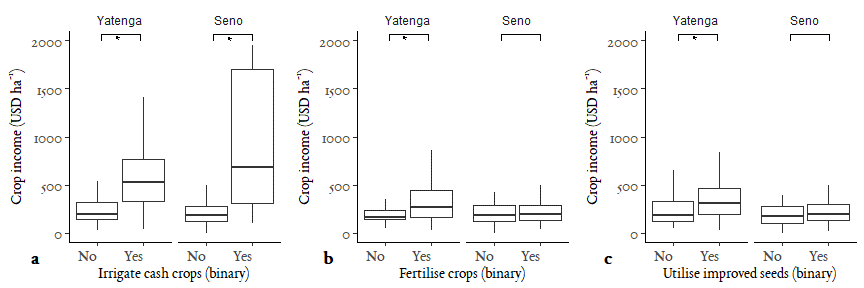
\includegraphics[width=1\textwidth]{figs_05/image2.png}
  \captionsetup{singlelinecheck = off, justification=justified}
  \caption{Gross crop income by practice adoption (irrigation, fertiliser and improved seeds) and province}
  \label{fig:05_1}
  %\small
  %\raggedright
  \vspace*{-3mm}
  \caption*{*Groups have differing central tendencies}
\end{figure}


Larger land sizes and higher rates of market participation in Yatenga province resulted in a higher median energy adequacy ratio and higher median crop income, in comparison to Seno (Table \ref{tab:05_2}). In Yatenga province, households at the median were potentially self-sufficient in energy needs; in Seno province, the median energy adequacy ratio was below sufficiency, with 80\% of energy needs met by home consumption of crops and animal-source foods. Livestock market participation was more common in Seno province, as was consumption of home-produced livestock products -- as shown in the higher adequacy ratio of protein from animal sources and higher median income from livestock products (Table \ref{tab:05_2}).

Off-farm income was common across provinces (67\% of households in Yatenga, 57\% of households in Seno), with the majority earning under US\$500 per household per annum. For those that did earn off-farm income, the central tendency of earnings was similar across provinces (median of US\$296 in Yatenga and US\$375 in Seno). Households in Yatenga generally had higher gross incomes, yet significantly less income from live animals (Table \ref{tab:05_2}). Control of income did not differ significantly by province, where the majority (85\%) of households had less than 10\% of income controlled by females. Households in Yatenga province tended to have a higher Progress out of Poverty Indicator score (PPI).



\begin{table}[H]
  \captionsetup{singlelinecheck = false, justification=justified} %left justify caption
  \caption{Summary of resources and farming activity of households (median and IQR)}
  \label{tab:05_2}
  \small
\begin{tabularx}{\textwidth}
  {
  p{\dimexpr 0.45\linewidth-2\tabcolsep}
  YYY}
%p{\dimexpr 0.23\linewidth-2\tabcolsep}
%p{\dimexpr 0.23\linewidth-2\tabcolsep}
%p{\dimexpr 0.09\linewidth-2\tabcolsep}}
\toprule
Characteristic & Yatenga & Seno & \\
 & (n = 200) & (n = 200) & \\
 \midrule
Household inhabitants (adult eq.) & 10.4 (5.4) & 6.8 (5.3) & * \\
Land area (ha) & 5.0 (4.1) & 3.5 (3.0) & * \\
Livestock holdings (TLUs)$^{\mathrm{a}}$ & 5.20 (4.8) & 5.1 (9.0) & NS \\
\arrayrulecolor{black!30}\midrule
Off-farm income (USD year$^{-1}$)$^{\mathrm{b}}$ & 83.25 (451.62) & 74.92 (416.24) & NS \\
Crop gross income (USD year$^{-1}$)$^{\mathrm{b}}$ & 354.56 (637.55) & 0.00 (8.11) & * \\
Live animal net income (USD year$^{-1}$)$^{\mathrm{b}}$ & 12.49 (97.90) & 60.84 (248.72) & * \\
Animal product net income (USD year$^{-1}$)$^{\mathrm{b}}$ & 0 (0) & 0 (0) & NS \\
Relative female control (\% income year$^{-1}$) & 0 (2) & 0 (0) & * \\
Progress out of Poverty Index score & 38 (14) & 31 (16) & * \\
\arrayrulecolor{black!30}\midrule
Number of crop species & 5 (2) & 3 (2) & * \\
Crop production diversity & 2 (1) & 2 (0) & * \\
Sorghum yield (kg ha$^{-1}$) & 225.0 (338.0) & 250.0 (250.0) & * \\
Millet yield (kg ha$^{-1}$) & 184.0 (350.0) & 217.0 (350.0) & NS \\
Maize yield (kg ha$^{-1}$) & 650 (985.0) & 720.0 (725.0) & * \\
Crop market participation (\% of total calories produced year$^{-1}$) & 41 (26) & 0 (1) & * \\
Crops consumed (kcal adequacy ratio adult equivalent$^{-1}$) & 1.00 (1.1) & 0.8 (0.7) & * \\
\arrayrulecolor{black!30}\midrule
Number of livestock species & 4 (2) & 4 (2) & NS \\
Livestock production diversity score & 1 (0) & 2 (1) & NS \\
Livestock market participation (\% of protein produced year$^{-1}$) & 0 (0) & 0 (3) & NS \\
Livestock products consumed (protein adult equivalent$^{-1}$ adequacy ratio) & 0.02 (0.02) & 0.15 (0.27) & * \\
\arrayrulecolor{black}\bottomrule
\end{tabularx}
\footnotesize
\raggedright
%\caption*{
*CI does not cross zero. Provinces have differing central tendencies\\
$^NS$CI crosses zero or model does not converge\\
$^a$Oxen = 1.42, cows = 1, camel = 1.1, horse = 0.9, donkey = 0.8, pigs = 0.3, sheep and goats = 0.2, chickens = 0.04\\
$^b$1 CFA = 0.001665 USD%}
\end{table}



\subsection{Determinants of food (in)security of access}

Households had differing perceptions of the severity and duration of food insecurity. In Yatenga province, the most common period of perceived shortage was between February and October (27\% of households). In Seno province 43\% of households perceived a shortage of food between June and October. Many households perceived that they had just enough food throughout the year (27\% in Yatenga and 20\% in Seno), and a few households considered themselves to be food secure throughout the year (8\% in Yatenga and 6.5\% in Seno). There was only one household per province that perceived a shortage in the period between November and February, where the majority of households considered themselves to be secure during this time. For the following analysis, the `flush' period can be considered as this period between November and February and the `lean' period as being more variable in duration and severity -- between February and October. Aid in the form of food or money was distributed in the study area. In Yatenga province, 40\% of households received aid, whereas in Seno province, only two households received aid. The most common period of aid provision was between June and October (results not shown).

The majority of households in the `lean' period were classified as either `severely food insecure' or `moderately food insecure' using the Household Food Insecurity Access Prevalence (HFIAP) indicator. In Yatenga province, approximately 31\% of households were classified as `severely food insecure' in the `lean' period, 41\% as `moderately food insecure', 17\% as `mildly food insecure' and 10\% as `food secure'. The food security status of households in Seno province was worse, with over 84\% of households classified as being `severely food insecure' in the `lean' period, 13\% classified as `moderately food insecure', 2\% classified as `mildly food insecure' and less than 2\% classified as `food secure'.

The HFIAS variable was modelled as a function of gross income (off-farm, crop and livestock), gendered control of income, energy adequacy, species diversity, whether aid was received and province of residence. There was a positive association between gross income and a higher food security of access status (i.e. not severely food insecure) in both provinces in the `lean' period; this association was stronger in Yatenga -- indicated by the significant interaction term (Table \ref{tab:05_3}). The number of livestock species kept was positively associated with a higher food security of access status in the `lean' period. Consumption adequacy, the number of crop species and receiving aid were not associated with food security of access in the `lean' period (Table \ref{tab:05_3}). Furthermore, there were no statistically significant associations identified for relative female control, higher food security status or the number of crop species cultivated in the `flush' period.



\begin{table}[H]
  \captionsetup{singlelinecheck = false, justification=justified} %left justify caption
  \caption{Household Food Insecurity Access (logistic regressions${\dag}$)}
  \label{tab:05_3}
  \small
\begin{tabularx}{\textwidth}%{@{}lYY@{}}
  {
p{\dimexpr 0.48\linewidth-2\tabcolsep}
Y Y}
%p{\dimexpr 0.26\linewidth-2\tabcolsep}
%p{\dimexpr 0.27\linewidth-2\tabcolsep}}
\toprule
Fixed effects & Lean period$^{\mathrm{a}}$ & Flush period$^{\mathrm{a}}$ \\
 \midrule
Intercept & -2.44 (-5.20, 0.04) & 1.08 (-1.76, 4.59) \\
Gross income (`000 USD year$^{-1}$) & 0.34 (0.08, 0.64) * & 0.16 (0.02, 0.36) * \\
Food consumed from own farm (kcal adequacy ratio adult equivalent$^{-1}$) & -0.18 (-0.45, 0.01) & 0.02 (-0.09, 0.15) \\
Number of crop species & 0.11 (-0.16, 0.37) & 0.09 (-0.18, 0.34) \\
Number of livestock species & 0.32 (0.10, 0.55) * & 0.08 (-0.12, 0.28) \\
Aid received$^{\mathrm{b}}$ & 0.08 (-0.82, 0.97) & 0.13 (-0.93, 1.17) \\
Province$^{\mathrm{c}}$ & -0.62 (-2.22, 1.11) & -0.63 (-2.30, 1.20) \\
\arrayrulecolor{black!30}\midrule
Gross income:province & -0.53 (-0.95, -0.17) * & \\
\arrayrulecolor{black}\bottomrule
\end{tabularx}
\footnotesize
\raggedright
%\caption*{
$^{\dag}$ Estimates are presented as posterior ${\upbeta}$ estimate and 95\% credible interval (CI)\\
* CI does not cross zero\\
$^a$Reference category is `severely food insecure of access'\\
$^b$Reference category for dichotomous variable is `no'\\
$^c$Reference category is Yatenga province\\%}
\end{table}



\subsection{Determinants of household diet diversity}

The household diet diversity score differed across periods and provinces. In general, diets were more diverse in the `flush' period and households in Yatenga province tended to have more diverse diets in the `lean' period than households in Seno province (intercepts and province coefficient in Table \ref{tab:05_4} and medians in Table \ref{tab:05_5}). Table \ref{tab:05_4} presents regression outputs for HDDS in both the `lean' and `flush' periods. In the `lean' period there are interactions between gross farm income, off-farm income and province, which makes the associations difficult to interpret from the combination of coefficients; these interactions are best visualised as marginal effects. Figure \ref{fig:05_2} presents the associations between gross farm income and diet diversity in the `lean' period. Gross farm income was positively associated with diet diversity in Yatenga province in the `lean' period, particularly for households that did not earn off-farm income. In Seno province these associations differ, where diet diversity in the `lean' period is predicted to increase as gross farm income increases -- only when off-farm income is also earned. Households that did not earn off-farm income in Seno province were predicted to decreased in diet diversity in the `lean' period as gross farm income increased.

Crop species diversity was also positively associated with diet diversity in the `lean' period -- regardless of province. This statistically significant association, however, did not persist when assessing crop production diversity (count of crop products in HDDS categories) -- which, by definition, has a closer association with HDDS.

We also assessed whether: a) the influence of farm income on diet diversity is mediated by female control, and b) food self-sufficiency is positively associated with diet diversity. However, female control of income and food self-sufficiency were not found to be associated with diet diversity in this study.



\begin{table}[H]
  \captionsetup{singlelinecheck = false, justification=justified} %left justify caption
  \caption{Household diet diversity (Mixed-effects negative binomial regressions${\dag}$)}
  \label{tab:05_4}
  \small
\begin{tabularx}{\textwidth}{@{}lYY@{}}
%  {
%p{\dimexpr 0.55\linewidth-2\tabcolsep}
%p{\dimexpr 0.24\linewidth-2\tabcolsep}
%p{\dimexpr 0.21\linewidth-2\tabcolsep}}
\toprule
 Fixed effects & Lean period & Flush period \\
 \midrule
Intercept & 1.26 (1.03, 1.50) * & 2.00 (1.78, 2.21) * \\
Gross farm income (`000 USD year$^{-1}$) & 0.01 (-0.06, 0.07) & 0.02 (-0.01, 0.04) \\
Off-farm income earned$^{\mathrm{a}}$ & 0.13 (0.01, 0.26) * & 0.05 (-0.03, 0.14) \\
Relative female control ({\textgreater} 40\% income year$^{-1}$) & 0.08 (-0.07, 0.22) & -0.04 (-0.16, 0.09) \\
Number of crop species & 0.05 (0.01, 0.09) * & 0.01 (-0.02, 0.04) \\
Number of livestock species & 0.00 (-0.03, 0.04) & 0.01 (-0.01, 0.04) \\
Province$^{\mathrm{b}}$ & -0.31 (-0.52, -0.09) * & -0.02 (-0.26, 0.22) \\
\arrayrulecolor{black!30}\midrule
Gross farm income:off-farm income earned & 0.03 (-0.05, 0.12) & \\
Gross farm income:province & -0.10 (-0.19, 0.00) * & \\
Off-farm income earned:province & 0.08 (-0.10, 0.25) & \\
Gross farm income:off-farm income earned:province & 0.16 (0.04, 0.28) * & \\
\arrayrulecolor{black}\bottomrule
\end{tabularx}
\footnotesize
\raggedright
%\caption*{
$^{\dag}$Estimates are presented as posterior ${\upbeta}$ estimate and 95\% credible interval (CI)\\
*CI does not cross zero\\
$^a$Reference category for dichotomous variable is `no'\\
$^b$Reference category is Yatenga province\\%}
\end{table}





\begin{figure}[H]
  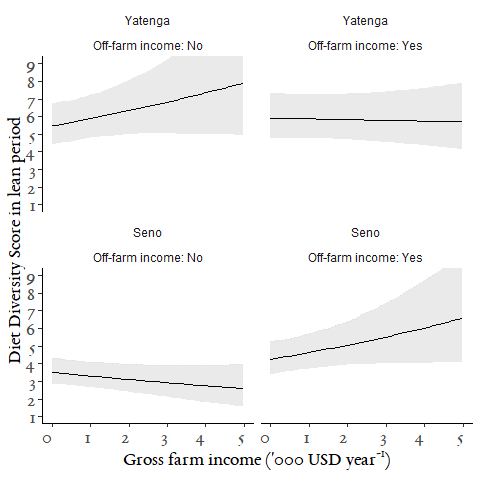
\includegraphics[width=0.5\textwidth]{figs_05/image3.png}
  \captionsetup{singlelinecheck = off, justification=justified}
    \caption{Household diet diversity dcore in the `lean' period. Marginal effects of gross income (`000 USD) by off-farm income and province; dashed lines indicate uncertainty of marginal effect estimates at a 95\% credible interval. All associations represented are statistically significant}
    \label{fig:05_2}
\end{figure}

The channel of access of food categories provides a disaggregated view of HDDS. In both provinces and periods, purchased diversity was a greater point of differentiation than farm-sourced diversity (Table \ref{tab:05_5}). The median number of purchased food categories was three times as much as own farm-sourced categories in the `lean' period and more than double own farm-sourced categories in the `flush' period. Farm-sourced categories were largely limited to the cereals and `pulses, legumes and nuts' categories, with some households having the addition of vegetables, eggs, meat and/or milk (results not shown).


\begin{table}
  \captionsetup{singlelinecheck = false, justification=justified}
  \caption{Summary of Household diet diversity score for households (HDDS; median and IQR)}
  \label{tab:05_5}
  \small
\begin{tabular}{L{7.3cm} C{3cm} C{3cm} C{1cm}} %Page is 14.3cm across %{\textwidth}{@{}lYYY@{}}
  %{
%p{\dimexpr 0.44\linewidth-2\tabcolsep}
%p{\dimexpr 0.2\linewidth-2\tabcolsep}
%p{\dimexpr 0.21\linewidth-2\tabcolsep}
%p{\dimexpr 0.15\linewidth-2\tabcolsep}}
\toprule
 & Seno (n = 200) & Yatenga (n = 200) &  \\
 \midrule
HDDS - lean period & 3.5 (3.0) & 6.0 (2.0) & * \\
HDDS - flush period & 8.0 (4.0) & 9.0 (1.0) & \\
HDDS from farm production - lean period & 1.0 (1.0) & 2.0 (2.0) & * \\
HDDS purchased - lean period$^{\mathrm{a}}$ & 3.0 (3.0) & 6.0 (2.0) & * \\
HDDS from farm production - flush period & 3.0 (2.0) & 3.0 (2.0) & * \\
HDDS purchased -- flush period & 7.0 (5.0) & 7.0 (2.0) & \\
\bottomrule
\end{tabular}
\footnotesize
\raggedright
%\caption*{
*Provinces have differing central tendencies\\
$^a$Observations with no purchased food in the `lean' period removed (n = 8 from Yatenga province)%}
\end{table}



At the aggregate level, the own-farm channel of food access had a limited association with diet diversity. This is understandable, where in the `lean' period, households in tended to source only one or two food categories from their farm (Table \ref{tab:05_5}). At the disaggregated level, the number of crop species cultivated is associated with diet diversity accessed through the own-farm channel in the `lean' period (Table \ref{tab:05_6}). In the `flush' period, both the number of crop and livestock species are associated with diet diversity accessed through the own-farm channel. These associations persisted when assessing crop and livestock production diversity instead of species diversity (results not shown).


\begin{table}
  \captionsetup{singlelinecheck = false, justification=justified}
  \caption{Household diet diversity accessed through own-farm channel (mixed-effects negative binomial regression${\dag}$)}
  \label{tab:05_6}
  \small
\begin{tabularx}{\textwidth}{@{}lYY@{}}
  %{
%p{\dimexpr 0.42\linewidth-2\tabcolsep}
%p{\dimexpr 0.29\linewidth-2\tabcolsep}
%p{\dimexpr 0.29\linewidth-2\tabcolsep}}
\toprule
Fixed effects & Lean period & Flush period \\
 \midrule
Intercept & -0.08 (-0.69, 0.52) & 0.75 (0.38, 1.13) * \\
Number of crop species & 0.11 (0.05, 0.18) * & 0.05 (0.00, 0.10) * \\
Number of livestock species & 0.03 (-0.03, 0.08) & 0.05 (0.01, 0.09) * \\
Province$^{\mathrm{a}}$ & 0.24 (-0.54, 1.04) & 0.26 (-0.18, 0.73) \\
\bottomrule
\end{tabularx}
\footnotesize
\raggedright
%\caption*{
$^{\dag}$Estimates are presented as posterior ${\upbeta}$ estimate and 95\% credible interval (CI)\\
*CI does not cross zero\\
$^a$Reference category is Yatenga province.%}
\end{table}



At the disaggregated level, there is greater uncertainty around the interactions between purchased diet diversity, farm income, off-farm income and province (Table \ref{tab:05_7}). At this disaggregated level we also see an association between the number of crop species cultivated and purchased diet diversity in the `lean' period. This association cannot be considered causal as the own-farm channel of food access is not represented in Table \ref{tab:05_7}. Rather, this result informs us that the purchased channel to diet diversity is not impeded by crop species diversity.

\begin{table}[H]
  \captionsetup{singlelinecheck = false, justification=justified}
  \caption{Household diet diversity accessed through purchased channel (mixed-effects negative binomial regression${\dag}$)}
  \label{tab:05_7}
  \small
\begin{tabularx}{\textwidth}{@{}lYY@{}}
  %{
%p{\dimexpr 0.55\linewidth-2\tabcolsep}
%p{\dimexpr 0.24\linewidth-2\tabcolsep}
%p{\dimexpr 0.21\linewidth-2\tabcolsep}}
\toprule
 Fixed effects & Lean period$^{\mathrm{a}}$ & Flush period \\
 \midrule
Intercept & 1.23 (1.01, 1.46) * & 1.81 (1.51, 2.12) * \\
Gross farm income (`000 USD year$^{-1}$) & 0.04 (-0.02, 0.09) & 0.00 (0.00, 0.00) \\
Off-farm income earned$^{\mathrm{b}}$ & 0.14 (0.01, 0.27) * & 0.05 (-0.05, 0.15) \\
Relative female control ({\textgreater} 40\% calories year$^{-1}$) & 0.07 (-0.09, 0.23) & -0.07 (-0.21, 0.06) \\
Number of crop species & 0.04 (0.00, 0.09) * & 0.02 (-0.02, 0.05) \\
Number of livestock species & -0.01 (-0.05, 0.02) & 0.01 (-0.02, 0.04) \\
Province$^{\mathrm{c}}$ & -0.35 (-0.52, -0.16) * & 0.00 (-0.37, 0.39) \\
\arrayrulecolor{black!30}\midrule
Gross farm income:off-farm income earned & -0.00 (-0.08, 0.07) & \\
Gross farm income:province & -0.05 (-0.12, 0.03) & \\
Off-farm income earned:province & 0.14 (-0.05, 0.33) & \\
Gross farm income:off-farm income earned:province & 0.09 (-0.02, 0.20) & \\
\arrayrulecolor{black}\bottomrule
\end{tabularx}
\footnotesize
\raggedright
%\caption*{
$^{\dag}$Estimates are presented as posterior ${\upbeta}$ estimate and 95\% credible interval (CI)\\
*CI does not cross zero\\
$^a$Observations with no purchased food in the `lean' period removed (n = 8 from Yatenga province)\\
$^b$Reference category for dichotomous variable is `no'\\
$^c$Reference category is Yatenga province.\\%}
\end{table}



\section{Discussion}

Our analysis shows that in both provinces, the ability to purchase food is what differentiates the more food secure households from their less food secure counterparts. This finding does not detract from the utility of subsistence production -- where consumption of own-farm food tended to cater for 91\% of the annual energy requirements in Yatenga province and 72\% in Seno province. Rather, purchasing power was the differentiating factor between households with food availability and those that are more food secure. This differentiation of households is most apparent in the dietary diversity indicator, where in both `flush' and `lean' periods, purchased food groups are more numerous than consumption of own-farm produced food groups (Table \ref{tab:05_5}). This is logical in this setting where at maximum, households could source nine of the twelve categories from their farm (including processing oil); realistically, households were observed to source two to three categories from their farm in the `flush' period (similar findings in \citealp{Some2018}). These farm-sourced categories were largely limited to the cereals and `pulses, legumes and nuts' categories. This finding is consistent with the majority of recent studies on the relative importance of purchased/farm-sourced foods (\citealp{Bellon2016}; \citealp{Koppmair2017325}; \citealp{Luckett20152479}; \citealp{Sibhatu201510657}; \citealp{Snapp2015}; and \citealp{Dillon2014}). Similarly, \citet{Jones2016}, while emphasising the importance of diverse farm production across wealth strata, noted that the relationship between production diversity and diet diversity may be mediated through income generation (and thus purchased food), as well as farm-sourced food groups. With a growing consensus, can it then be concluded (as implicit in the aims of \citealp{FAO2016a}) that food insecurity will be eradicated by doubling the `agricultural productivity and incomes of small-scale producers' through on-farm means and off-farm employment/business? Food security is not simply limited to an individual's capacity to access calories. Other important dimensions of food security include: protein and micro-nutrient intake, resilient agricultural practices, maintaining genetic diversity of plants and animals, and maintaining access to culturally relevant foods (\citealp{FAO2008}). Further, the allocation of scarce household resources is not solely dedicated to achieving food security. Households use their income to pursue multiple goals (e.g. education), and the allocation of resources depends on needs (including food security and other higher order needs) and complex intra-household dynamics (\citealp{Kazianga2017}; \citealp{Galie2015}).

\subsection{Towards a pathway model of food security}

The potential pathways from food and income availability to food security analysed in this study are represented diagrammatically in Figure \ref{fig:05_3}. The diagram includes farm resources and activities from Table \ref{tab:05_1} and Figure \ref{fig:05_1} on the left-hand-side, representing the basis for food production. Both market and subsistence (own-farm) channels to food security are represented in a flow (indicated by arrows) from the left-hand-side towards the right-hand-side. Market participation, off-farm income and aid all contribute to net income. Mediated through expenditure and consumption decisions, these two channels of food access (purchased and own-farm) then have a bearing on the availability of food, energy access, diversity of food access, access to culturally relevant foods, and stability of food security over time (right-hand-side of Figure \ref{fig:05_3}). The pathways from food and income availability to food security may also influence the pattern of food utilisation within a household. This dimension of food security, however, is beyond the scope of this study.

\begin{figure}[H]
  \captionsetup{singlelinecheck = false, justification=justified}
  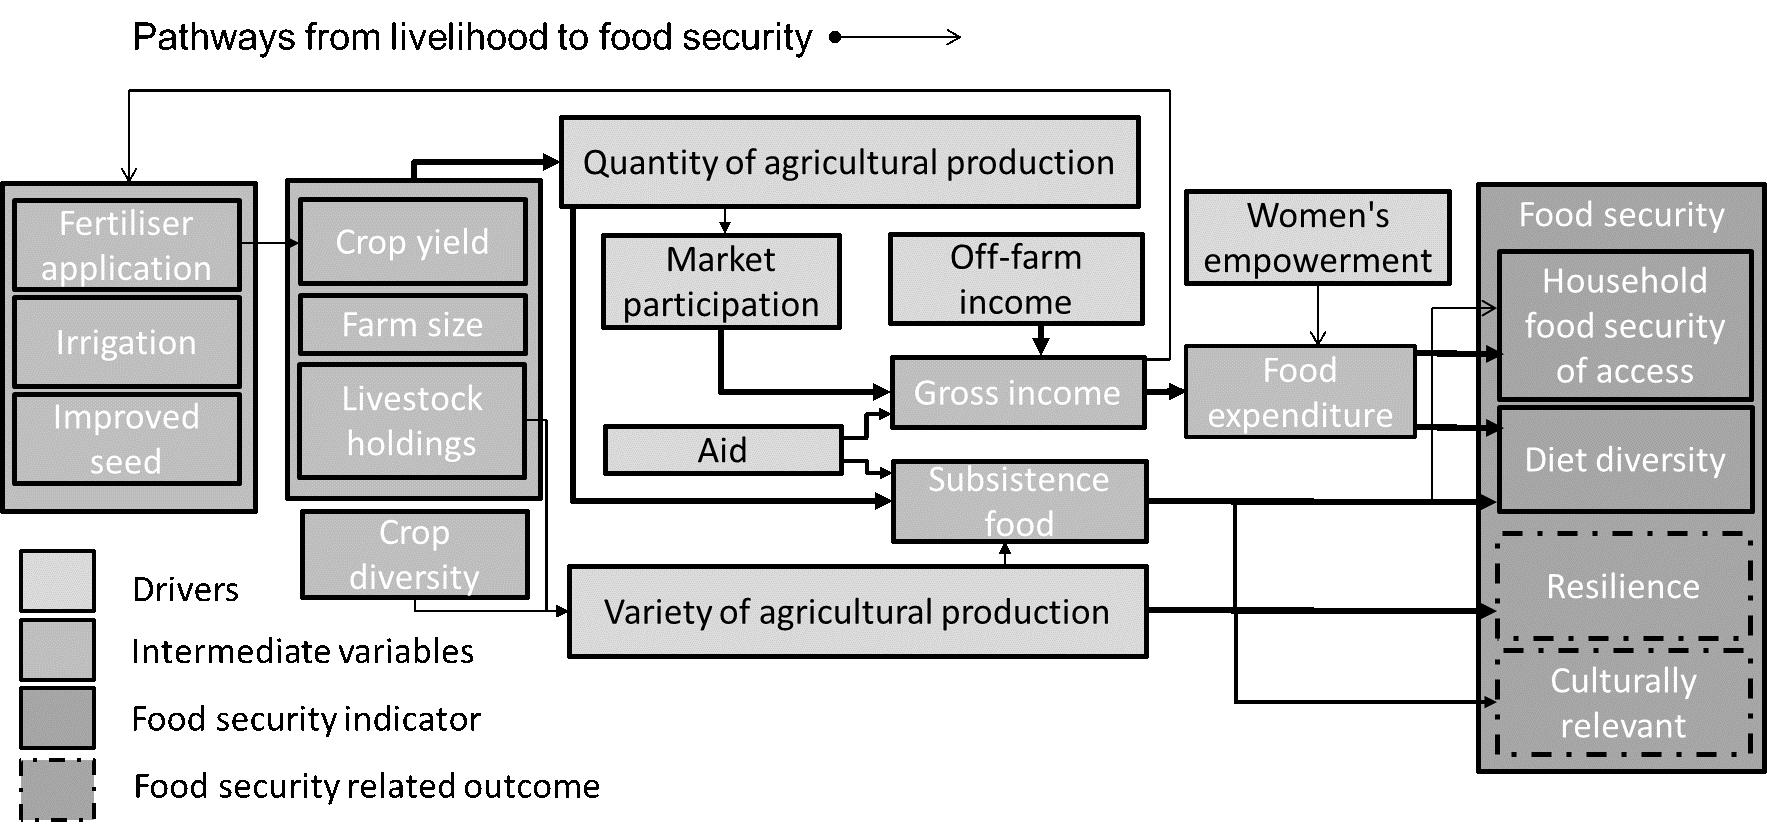
\includegraphics[width=1\textwidth]{figs_05/image4.png}
  \caption{Pathways to food security outcomes (adapted from \citealp{Jones2016})}
  \label{fig:05_3}
\end{figure}

The relationship between crop diversity and the diversity of food access is a central area of inquiry in the literature. Previous studies have used this relationship to draw conclusions on whether to reduce hidden hunger by supporting market-oriented interventions (upper drivers in Figure \ref{fig:05_3}) or by promoting agrobiodiversity (lower driver in Figure \ref{fig:05_3}). Our results suggest that these goals do not have to be mutually exclusive. Both gross income and livestock species diversity, for example, are associated with improved food security of access. Similarly, both gross farm income and crop species diversity were associated with more diverse diets. Considering the implications of this more generally, livestock keeping -- as part of a diversified portfolio -- provides soil health benefits through the recycling of nutrients, as well as reducing livelihood risk by acting as a means to store capital (\citealp{Moll2005}; \citealp{Slingerland2000}). Similarly, diversified crop production can contribute to pest and disease management; reduce the market risk of volatile prices, and; can also be a part of a soil health strategy (e.g. nitrogen fixation or cover cropping to reduce erosion; \citealp{Lin2011}). Each of these benefits can improve the resilience of a farm and a livelihood (contributing to stability in Figure \ref{fig:05_3}), specifically in relation to climatic or economic shocks.

The majority of households cultivated sorghum and millet. Access to such culturally relevant and nutritious foods is not guaranteed in the future (\citealp{Schipanski2016}; \citealp{Pingali2015}; \citealp{Remans2014}). The global trend of increasing food homogeneity (e.g. \citealp{Khoury2014}) has already resulted in traditional, lower yielding grains such as tef (Eragrostis tef), millet (\textit{Pennisetum glaucum L}. and \textit{Eleusine coracana L}) and sorghum (Bicolour) being substituted with maize (\textit{Zea mays L.}), traditional vegetables replaced with market vegetables, and narrowed livestock genetic resources. The potential trade-offs between energy availability, resilience and the availability of culturally relevant and nutritious foods need to be considered to be able to optimise all aspects of food security. These trade-offs could be addressed -- in part -- by increased investment in locally relevant breeding (\citealp{Sibhatu201510657}) and the coupling of soil health education with fertiliser-based intensification programs (\citealp{Fonte2012}). Plant breeding can work to optimise yields and micro-nutrient bioavailability (increasing translocation and reducing inhibition) of locally relevant crops; and soil health can maintain/increase yields and improve soil micro-nutrient availability for the plants and ultimately the household (\citealp{DeValenca2017}; \citealp{Slingerland2006}).

The `income pathway' to improved food security has not been fully captured in all its complexity in this study. We observed significant differences in median crop income based on practice adoption. This relationship may be bi-directional, with higher incomes allowing practice adoption (represented as an arrow from gross income to practices on the left-hand-side of Figure \ref{fig:05_1}), and practice adoption increasing crop incomes. We also observed associations between gross income and food security (food security of access and diet diversity; Tables \ref{tab:05_3} and \ref{tab:05_4}). These associations differed substantially by province and whether off-farm income was earned (in the case of diet diversity). In this study, however, we did not identify any associations or interactions between female control of income and food security -- which by no means negates the reality that intra-household dynamics influence food access or food utilisation (e.g. \citealp{Mason2015}).

Off-farm income was more common in Yatenga (67\% of households in Yatenga compared to 57\% in Seno), but proved to be a greater differentiating factor in Seno. Having a wage or business income is an apparent advantage over a reliance on agriculture (\citealp{Reardon1992}). In Seno this advantage provides a pathway to a greater variety of food categories in the `lean' period -- when households are at their most vulnerable. From a policy and intervention perspective, there are macro-economic factors, regional comparative advantages and a range of other elements that drive the opportunities to engage in employment or business. With a growing rural population there is a need to improve rural non-farm opportunities (e.g. \citealp{Jayne2014}; \citealp{Haggblade2010}; \citealp{Tiffen2003}). This finding suggests that interventions to stimulate such opportunities can be targeted at specific regions or communities to improve household food security. A challenge that may arise in the process of stimulating off-farm opportunities, however, is that the individuals that capture them may not be the most in need; evidence suggests that wealthier households have a greater capacity to gain employment or invest in a non-farm business (\citealp{Davis2010}; \citealp{Haggblade2010}; \citealp{Reardon1992}). The complexities of the labour market are such that not only do the opportunities have to exist, but there also needs to be the availability of quality education options (\citealp{Jayne2014}) and functioning land tenure, credit and insurance markets (\citealp{Barrett2001}).

Aid (a potential driver of improved food security in Figure \ref{fig:05_3}) was received by a small portion of households in Yatenga province. There was no significant difference in food security status between recipients of aid and other respondents. This is not enough, however, to conclude whether this aid was effective in improving the food security of these households.

The experimental design of this study allowed us to improve our understanding of the causal pathways to improved food security in two subtly contrasting communities in drought prone regions of Burkina Faso. There are, however, some methodological limitations to our approach. Firstly, the sampling of this study was limited to eight villages within seven departments with some departments of Yatenga province excluded from sampling due to safety concerns. Conflict has been identified as an important driver of food insecurity (\citealp{FAO2018}) and so the results of this study cannot be taken to be representative of northern Yatenga. The limitation in sampling, however, necessitated the use of 1) weightings to correct the representativeness of our study and 2) a power analysis to assess the risk of Type II errors. A post-hoc analysis indicated that at a power of 0.8 (20\% risk of Type II error), these data allowed the detection of small differences in central tendency (Cohen's d {\textless} 0.2; results not tabulated elsewhere). Secondly, we enumerated food security indicators and farm production/marketing based on respondent recall. The complexity and length of recall may have negatively impacted measurement precision and item non-response (\citealp{Beegle2012}). To counteract this, we designed the survey to minimise respondent fatigue and we trained enumerators to cross-check responses to more complex questions. These design features, unfortunately, did not enable us to enumerate the cost of crop production -- which suffered from item non-response. Thirdly, as identified by \citet{Some2018}, we interviewed the household head on-farm activities -- potentially underestimating production diversity.

The food security status of households is most substantially and positively influenced by a household's ability to purchase food. This finding should not detract from the essential role played by subsistence production. Rather, market-orientated agriculture and production for home consumption, as shown by households in this study, can be combined as part of a broader livelihood strategy. Such livelihood strategies can improve food access and the stability of food security in both the `flush' and `lean' periods.

\section{Acknowledgments}

We thank the field team for their dedication and the participating rural households for their candor. This study was made possible by the support of the American People provided to the Feed the Future Innovation Lab for Sustainable Intensification through the United States Agency for International Development (USAID). The contents are the sole responsibility of the authors and do not necessarily reflect the views of USAID or the United States Government. Program activities are funded by the United States Agency for International Development (USAID) under Cooperative Agreement No. AID-OAA-L-14-00006. Also support by the CGIAR Research Program on Livestock is gratefully acknowledged.
